\documentclass{article}
\usepackage{listings} % 引入代码展示宏包
\usepackage{xcolor}
\lstset{
  backgroundcolor=\color{gray!10},      % 背景色:浅灰色
  basicstyle=\ttfamily\footnotesize,    % 基本样式:等宽字体,小号字体大小
  breakatwhitespace=false,              % 是否只在空白处自动断行
  breaklines=true,                      % 自动断行
  captionpos=b,                         % 标题位置:底部
  commentstyle=\color{green},           % 注释样式:绿色
  deletekeywords={...},                 % 删除的关键字
  escapeinside={\%*}{*)},               % LaTeX代码内嵌的转义符
  extendedchars=true,                   % 启用非ASCII字符
  frame=single,                         % 边框样式:单线边框
  keepspaces=true,                      % 保持空格,有助于保持代码的缩进
  keywordstyle=\color{blue},            % 关键字样式:蓝色
  language=bash,                        % 代码语言:Bash(Linux命令行)
  morekeywords={*,...},                 % 添加的关键字
  numbers=left,                         % 行号位置:左侧
  numbersep=5pt,                        % 行号与代码的距离
  numberstyle=\tiny\color{gray},        % 行号样式:小号字体,灰色
  rulecolor=\color{black},              % 边框颜色:黑色
  showspaces=false,                     % 不显示空格标记
  showstringspaces=false,               % 字符串中不显示空格标记
  showtabs=false,                       % 不显示制表符标记
  stepnumber=1,                         % 行号步进:每行显示
  stringstyle=\color{purple},           % 字符串样式:紫色
  tabsize=2,                            % 制表符大小
  title=\lstname                        % 显示文件名
}
\usepackage{multirow}
\usepackage{pgfplots}
\usepackage{ifthen}
\usepackage[UTF8]{ctex}
\usepackage[left=3.18cm,right=3.18cm,top=2.54cm,bottom=2.54cm]{geometry}
\geometry{a4paper}
\usepackage{tikz}
\usetikzlibrary{chains}
\newcommand{\diff}{\mathop{}\!\mathrm{d}}
\usepackage{appendix} 
\usepackage{diagbox}
\usepackage{pdfpages}
\usepackage{subcaption}
\usepackage{algorithm}
\usepackage{algpseudocode}
\renewcommand{\algorithmicrequire}{\textbf{Input:}}  
\renewcommand{\algorithmicensure}{\textbf{Output:}}  
\usepackage{amsmath}
\usepackage{amsthm}
\DeclareMathOperator{\sigm}{sigm}
\usepackage{graphicx} 
\usepackage{float}
\renewcommand{\vec}[1]{\boldsymbol{#1}}
\usepackage{amssymb}
\usepackage{booktabs} 
\usepackage{hyperref}
\usepackage{titlesec}
\usepackage{caption}
\captionsetup{font={small,bf}} 
\bibliographystyle{plain}
\newtheorem{definition}{定义}
\newtheorem{lemma}{引理}
\newtheorem{theorem}{定理}
\DeclareMathOperator{\Ima}{Im}
\DeclareMathOperator{\Rank}{rank}
\begin{document} \pingfang
\begin{center}
\textbf{\huge Parallel Desktop的安装和使用}
\end{center}
\begin{center}
    \textbf{\large \textbf{学号: \quad 姓名:王士博 \quad 指导教师:}}
\end{center}
\hrulefill
\section{实验环境和相关配置}
\begin{itemize}
    \item 1.宿主操作系统:macOS
    \item 2.虚拟机软件:Parallel Desktop 19 Business Edition
    \item 3.虚拟机操作系统:Ubuntu 20.04
    \item 4.本实验使用macOS系统,可以为以后使用macOS的同学提供一些参考;鉴于实验参考书中使用的Centos操作系统,本实验报告提供一些Ubuntu的使用方法
\end{itemize}
\section{实验目的和要求}
\begin{itemize}
    \item 1.安装Parallel Desktop,并且完成相关的配置。
    \item 2.建立虚拟机集群,首先要求能上网,掌握如何创建、克隆和管理虚拟机。要求建立三个虚拟机,实现相互发送和接收数据包。
    \item 3.了解SSH的基本使用。要求实现三台机器之间的无密码互访,如,master可以无密码远程登录slave1 和slave2。
    \item 4.使用ssh secure file transfer cliet实现windows主机与linxu虚拟机文件互传,使用ssh sucure shell client 实现在Windows上远程登录访问服务器。
\end{itemize}
\section{实验内容}
\subsection{安装Parallel Desktop}
\indent 从官网上下载Parallel Desktop的镜像文件,然后进行安装,基本全为默认。
\subsection{建立和克隆虚拟机}
\indent Parallel Desktop的虚拟机安装过程较为便捷,如果想要快速安装可以直接选取图\ref{fig:1}中
提供的相关系统,直接进行安装,安装默认的是最新版本,如果想要使用之前版本,可以在官网下载镜像然后通过
镜像进行安装。
\begin{figure}[H]
    \centering
    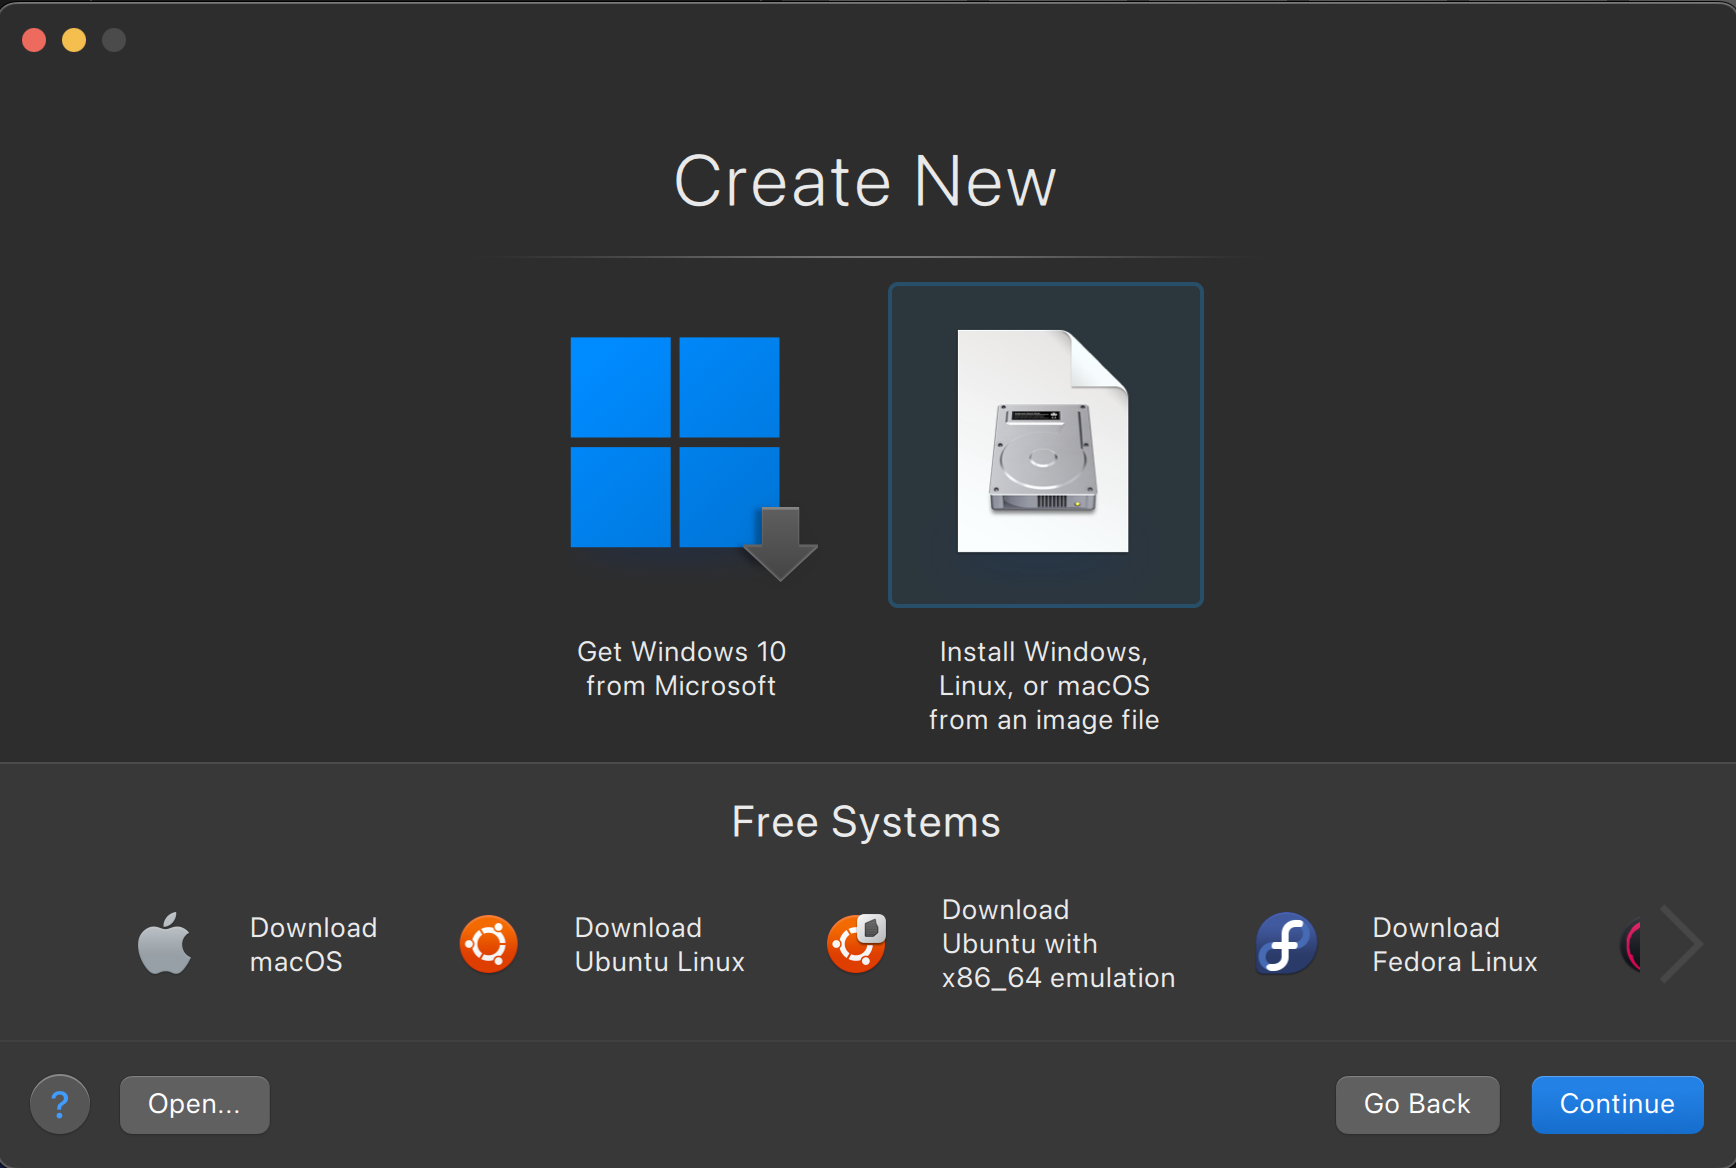
\includegraphics[width=0.7\textwidth]{image.png}
    \caption{Parallel Desktop的虚拟机安装界面}
    \label{fig:1}
\end{figure}
\indent 安装时还可以调整分配给虚拟机的硬件资源,如内存、CPU核心数、磁盘空间等,如图\ref{fig:2}所示
,如果有个人的需要可以进行调整否则直接全部默认即可。
\begin{figure}[H]
    \centering
    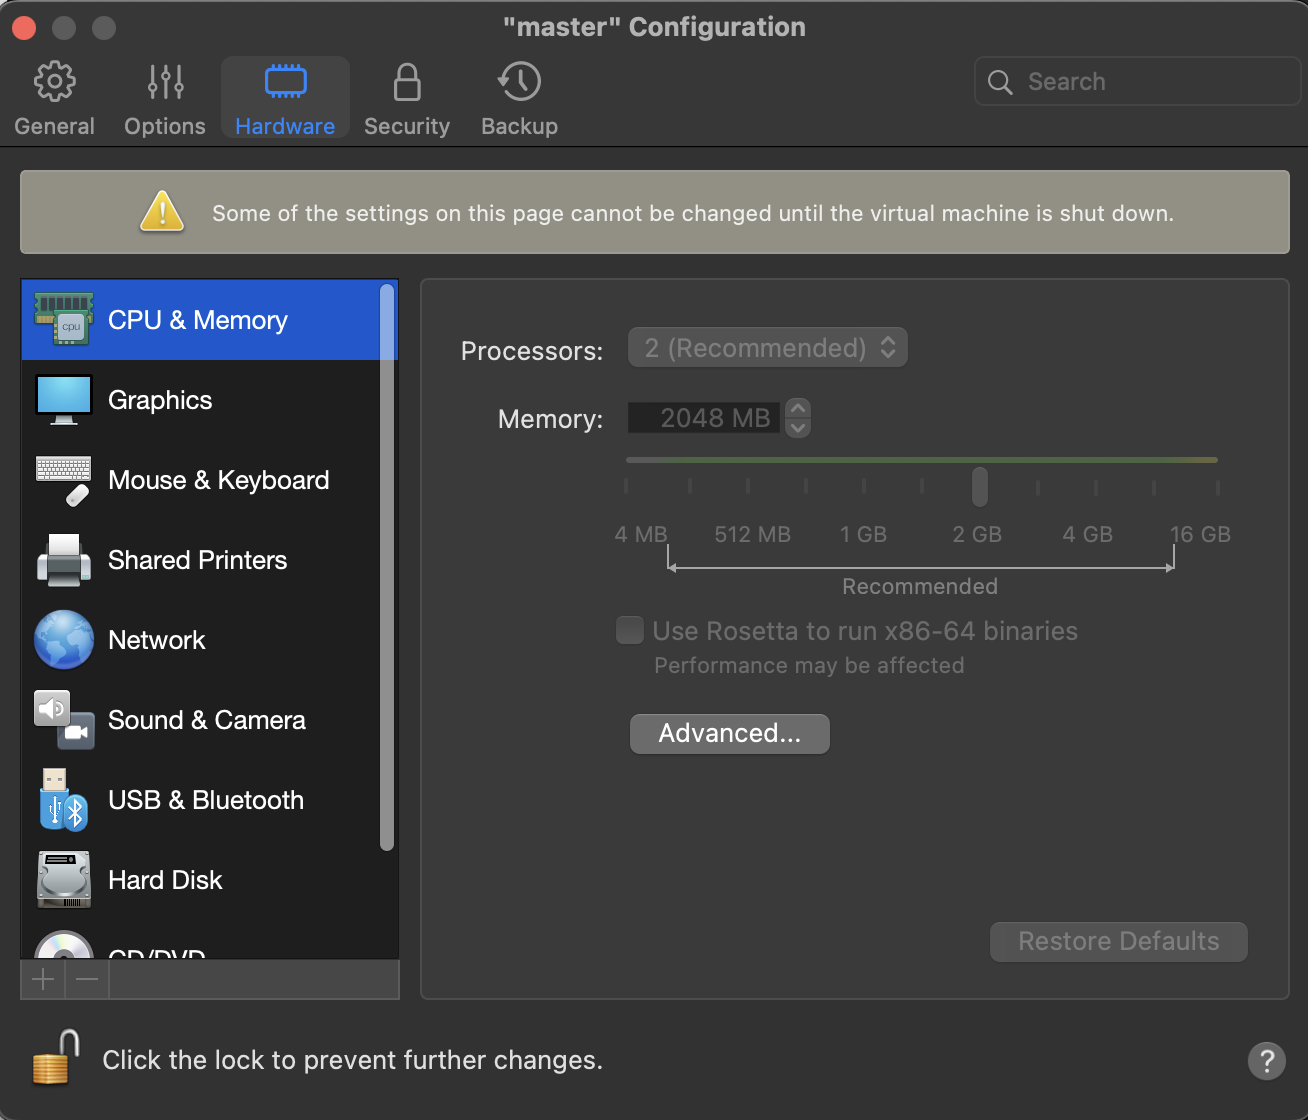
\includegraphics[width=0.6\textwidth]{image1.png}
    \caption{Parallel Desktop的虚拟机配置界面}
    \label{fig:2}
\end{figure}
\indent 安装完成后,可以进行虚拟机的克隆,如图\ref{fig:3}所示,直接复制两个相同的虚拟机然后双击添加到
Parallel Desktop中即可。
\begin{figure}[H]
    \centering
    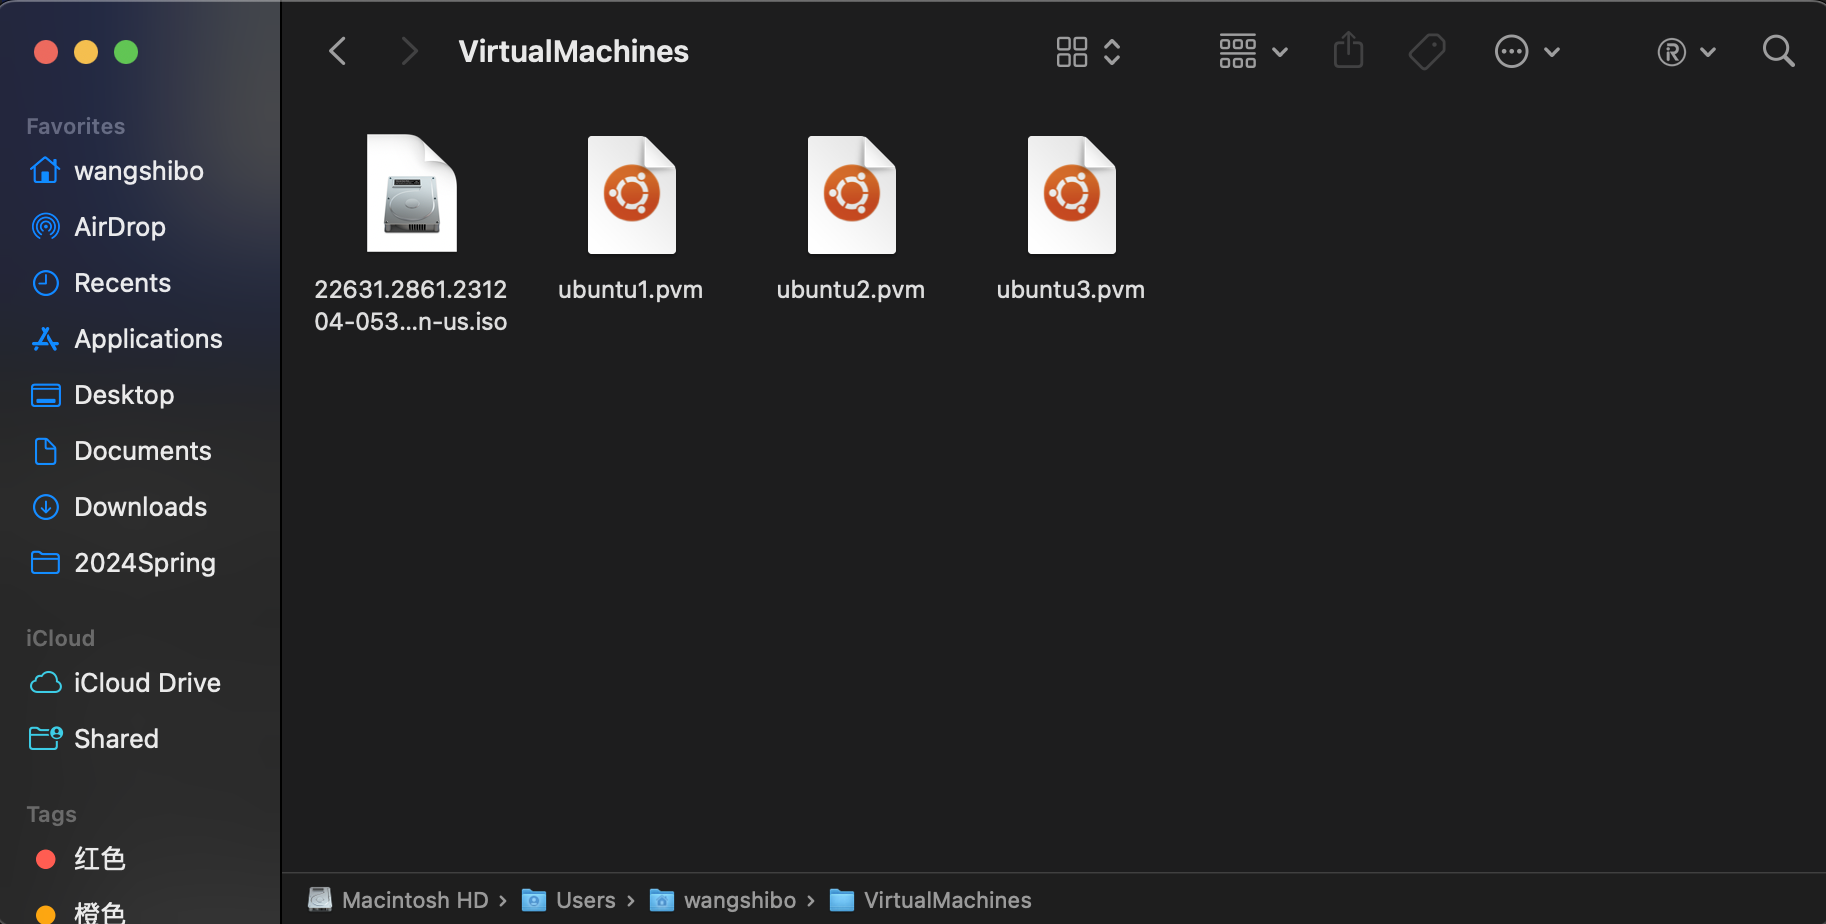
\includegraphics[width=0.6\textwidth]{image2.png}
    \caption{克隆虚拟机}
    \label{fig:3}
\end{figure}
\section{配置虚拟机网络}
\indent 虚拟机集群的组网方式使用了Parallel Desktop提供的共享网络模式,在VMware中也被称为NAT模式。
在这种模式下,宿主电脑和虚拟机集群在同一个局域网中(内网),介入到这个局域网的网卡使用私有IP地址进行
相互的通信,并且
宿主电脑相当于路由器,起到网关的作用,虚拟机通过宿主电脑访问互联网。

\indent 如果想要创建虚拟机集群,那么就要使用静态IP分配,不可以使用DHCP(动态IP分配),因为要
固定虚拟机之间的通信地址,如果每一次重启虚拟机集训或者宿主机器都会动态分配IP地址那么就需要重新
配置虚拟机集群的网络。拟使用下面的静态IP分配方式,宿主电脑提供一个192.168.1.0/24的网段,最多可
供253台虚拟机使用(除去全0的网段,为1的网关,全为1的广播地址)。
\begin{table}
    \centering
    \caption{静态IP分配表}
    \begin{tabular}{@{}lccc@{}}
        \toprule
        虚拟机名称 & IP地址 & 子网掩码 & 网关 \\ \midrule
        master & 192.168.1.10 & 255.255.255.0 & 192.168.1.1 \\
        slave1 & 192.168.1.11 & 255.255.255.0 & 192.168.1.1 \\
        slave2 & 192.168.1.12 & 255.255.255.0 & 192.168.1.1 \\
        \bottomrule
    \end{tabular}
\end{table}

\noindent 配置虚拟机的网络需要配置如下两个方面(三台机器的配置几乎相同,这里只介绍master的配置):
\begin{itemize}
    \item \textbf{1.配置虚拟机的静态IP地址:}Ubuntu的网络配置文件存放位置不同于Centos,存放在
    /etc/netplan/目录下,文件名为00-intsaller-config.yaml,首先使用ifconfig指令查看链接局域网
    的网卡名称,然后使用vim编辑器打开00-installer-config.yaml文件,修改相关文件内容,在进行之前需要先
    使用cp命令对文件进行备份,修改完成后使用netplan apply使得修改生效并且使用ifconfig查看是否修改成功。
    下面是修改的相关代码和文件内容。
    \begin{lstlisting}[caption={配置静态IP指令}]
parallels@master:~$ sudo su
[sudo] password for parallels: 
root@master:/home/parallels# ifconfig -a
enp0s5: flags=4163<UP,BROADCAST,RUNNING,MULTICAST>  mtu 1500
        inet 10.200.1.10  netmask 255.255.255.0  broadcast 10.200.1.255
        inet6 fe80::21c:42ff:febf:5095  prefixlen 64  scopeid 0x20<link>
        inet6 fdb2:2c26:f4e4:0:c36c:c129:57e0:4392  prefixlen 64  scopeid 0x0<global>
        inet6 fdb2:2c26:f4e4:0:21c:42ff:febf:5095  prefixlen 64  scopeid 0x0<global>
        ether 00:1c:42:bf:50:95  txqueuelen 1000  (Ethernet)
        RX packets 2344  bytes 772011 (772.0 KB)
        RX errors 0  dropped 0  overruns 0  frame 0
        TX packets 915  bytes 94756 (94.7 KB)
        TX errors 0  dropped 0 overruns 0  carrier 0  collisions 0
root@master:/home/parallels# cd /etc/netplan
root@master:/etc/netplan# cp 00-installer-config.yaml 00-installer-config.yaml_backup
root@master:/etc/netplan# vim 00-installer-config.yaml
root@master:/etc/netplan# netplan apply
** (generate:32379): WARNING **: 14:21:39.983: `gateway4` has been deprecated, use default routes instead.
See the 'Default routes' section of the documentation for more details.
root@master:/etc/netplan# ifconfig -a
enp0s5: flags=4163<UP,BROADCAST,RUNNING,MULTICAST>  mtu 1500
        inet 192.168.1.10  netmask 255.255.255.0  broadcast 192.168.1.255
        inet6 fe80::21c:42ff:febf:5095  prefixlen 64  scopeid 0x20<link>
        ether 00:1c:42:bf:50:95  txqueuelen 1000  (Ethernet)
        RX packets 2361  bytes 774788 (774.7 KB)
        RX errors 0  dropped 0  overruns 0  frame 0
        TX packets 975  bytes 101247 (101.2 KB)
        TX errors 0  dropped 0 overruns 0  carrier 0  collisions 0       
    \end{lstlisting}
    \begin{lstlisting}[caption={修改后的00-installer-config.yaml文件内容}]
network:
version: 2
renderer: NetworkManager
ethernets:
    enp0s5:
    dhcp4: no
    dhcp6: no
    addresses: [192.168.1.10/24]
    gateway4: 192.168.1.1
    nameservers:
        addresses: [8.8.8.8, 114.114.114.114]
    \end{lstlisting}
    \indent 可以看到上面的虚拟机的IP地址,网关已经修改,对剩下的两台虚拟机做同样的操作即可。
    \item \textbf{2.配置虚拟机的hostname和IP地址的映射关系:}
    对于虚拟机集群之间,可以直接使用IP地址进行通信,但是对于程序员,还是给每一个电脑取一个名字
    比较好记忆和维护,所以需要配置hostname和IP地址的映射关系,这里使用/etc/hosts文件进行配置。
    \begin{lstlisting}[caption={配置hostname和IP地址的映射关系指令}]
root@master:/etc/netplan# cd /
root@master:/# cd /etc
root@master:/etc# vim hostname
root@master:/etc# hostname
master
root@master:/etc# vim hosts
    \end{lstlisting}
    \begin{lstlisting}[caption={修改后的hosts文件内容}]
127.0.0.1 localhost
127.0.1.1 ubuntu-linux-22-04-desktop
192.168.1.10 master
192.168.1.11 slave1
192.168.1.12 slave2
# The following lines are desirable for IPv6 capable hosts
::1     ip6-localhost ip6-loopback
fe00::0 ip6-localnet
ff00::0 ip6-mcastprefix
ff02::1 ip6-allnodes
ff02::2 ip6-allrouters      
    \end{lstlisting}
    \indent 对剩下的两台虚拟机做同样的操作,然后就可以开始测试了。
\end{itemize}
\section{测试虚拟机集群对互联网和内网虚拟机之间的访问性}
\indent 首先测试虚拟机集群对互联网的访问性,使用ping命令给baidu.com发送ICMP报文,然后在使用
ping命令测试对slave1和slave2的访问性,如图\ref{fig:4}所示,可见完成了实验目标。
\begin{figure}[H]
    \centering
    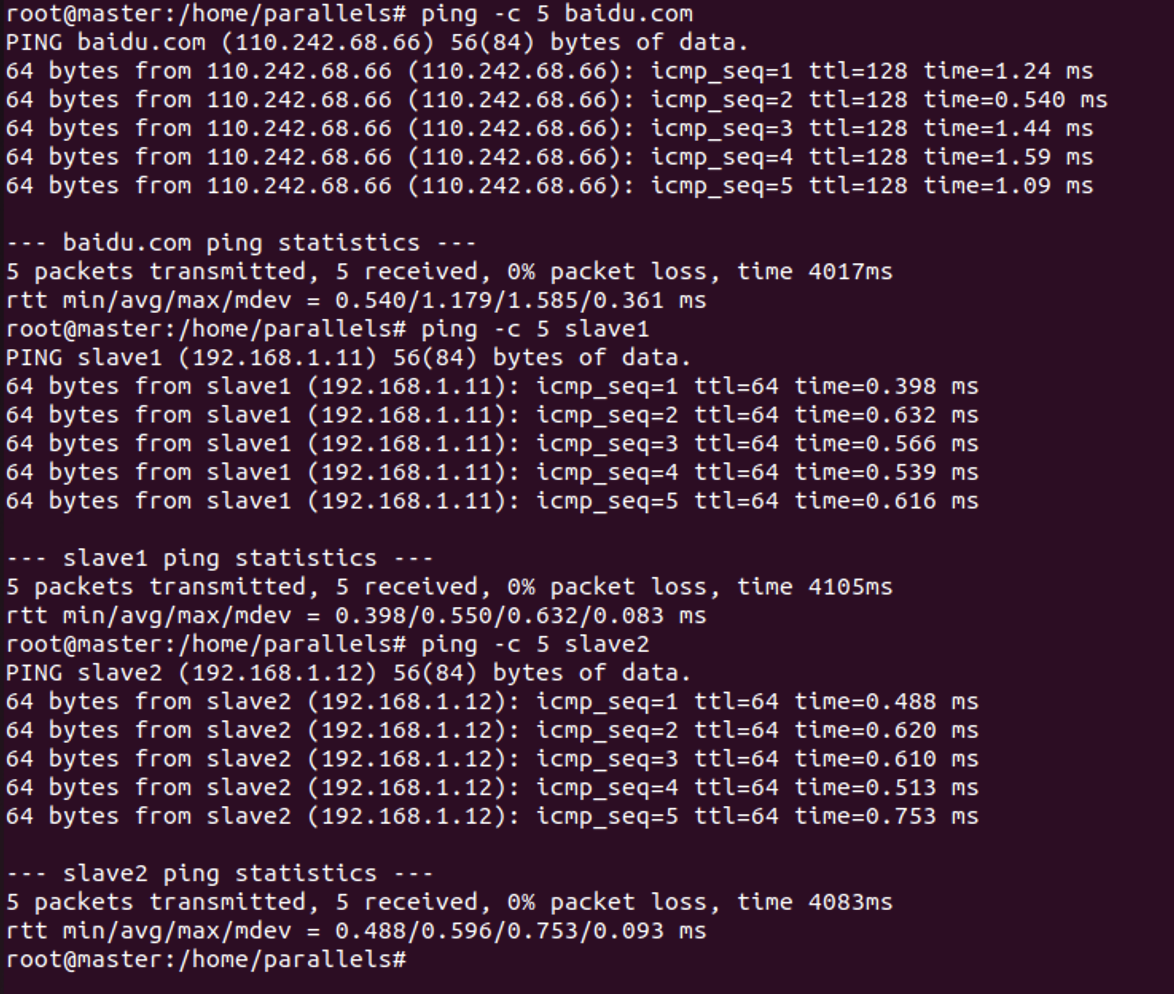
\includegraphics[width=0.6\textwidth]{image3.png}
    \caption{测试虚拟机集群对互联网和内网虚拟机之间的访问性}
    \label{fig:4}
\end{figure}
\section{ssh实现无密码访问}
\indent 

\section{rsh实现无密码访问}
\indent 
\section{title}
\end{document}